\documentclass[tikz, border=2mm]{standalone}

\usetikzlibrary{positioning,shapes,arrows,backgrounds,external,fit}
\usepackage[T1]{fontenc}
\usepackage[utf8]{inputenc}
\usepackage{lmodern}

\tikzset{
    BlockCPU/.style={draw,thick, fill=blue!20, rectangle},
    BlockAltre/.style={draw,thick, fill=blue!35, rectangle},
    Periferic/.style={ellipse, draw, fill=blue!15},
    Registre/.style={rectangle, draw, fill=blue!5},
    Nom/.style={font=\normalsize\sffamily,text centered, minimum size=1cm, text width=1.5cm}}

\begin{document}

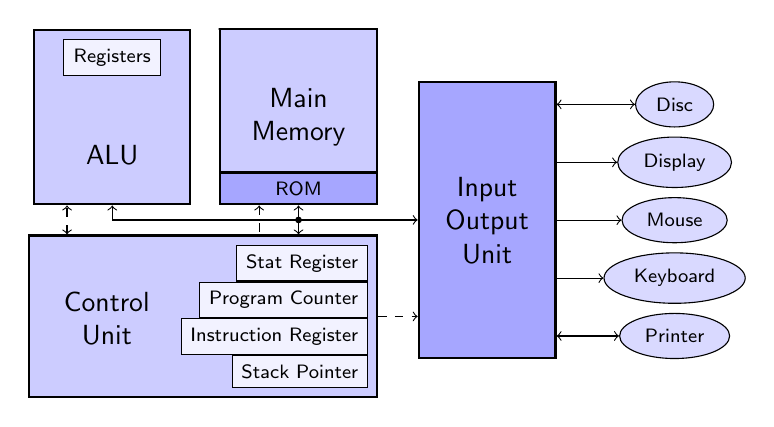
\begin{tikzpicture}[font={\sffamily\scriptsize}]

\node[Registre, anchor=south east] (SP) at (4.3,0.1) {Stack Pointer};
\node[Registre, anchor=south east] (IR) at (SP.north east) {Instruction Register};
\node[Registre, anchor=south east] (PC) at (IR.north east) {Program Counter};
\node[Registre, anchor=south east] (SR) at (PC.north east) {Stat Register};
\node[Nom, left=3mm of PC.south west] (UC) {Control Unit};

\begin{pgfonlayer}{background}
\node[BlockCPU,fit=(UC) (SR) (SP)] (UC2) {};
\end{pgfonlayer}{background}

\node[Nom,above right=5mm and 2mm of UC2.north west, anchor=south west] (UA) {ALU};
\node[Registre, above= 5mm of UA, text width=1cm, text centered] (Reg) {Registers};
\begin{pgfonlayer}{background}
\node[BlockCPU,fit=(Reg) (UA)] (ALU) {};
\end{pgfonlayer}{background}

\node[BlockAltre,minimum width=2cm,anchor=south east] (ROM) at (UC2.east|-ALU.south) {ROM};
\node[Nom,text width=1.5cm] (RAM) at (ROM|-ALU) {Main Memory};
%\node[Registre,text width=1cm, below=0.5mm of RAM, anchor=north,text centered] (Dades) {Data};
%\node[Registre,text width=1cm, below=1mm of Dades, text centered] (Codi) {Code};

\begin{pgfonlayer}{background}
\filldraw[thick,fill=blue!20] ([xshift=.5\pgflinewidth]ROM.north west) |- (ROM.west|-ALU.north) -|([xshift=-.5\pgflinewidth]ROM.north east);
\end{pgfonlayer}{background}
\node[BlockAltre,Nom,text width=1.5cm, text centered,minimum width=1.5cm, minimum height=3.5cm,above right=5mm and 5mm of UC2.south east,anchor=south west] (ES) {Input\\Output\\Unit}; 
\node[Periferic,right=15mm of ES.south east,anchor=south] (Impressora) {Printer};
\node[Periferic,anchor=north] (Disc) at (Impressora|-ES.north) {Disc};
\node[Periferic] (Ratoli) at (ES-|Disc) {Mouse};
\path (Disc) -- node[Periferic] (Pantalla) {Display} (Ratoli) -- node[Periferic] (Teclat) {Keyboard} (Impressora);
\draw[<->,dashed] ([xshift=5mm]UC2.north west) -- ([xshift=5mm]UC2.north west|-ALU.south);
\draw[<->] (ROM.south) -- node[coordinate] (punt) {} (ROM|-UC2.north);
\filldraw (punt) circle(1pt);
\draw[->] (punt) -| (ALU.south);
\draw[->] (punt) -- (punt -| ES.west);
\draw[<-,dashed] ([xshift=-5mm]ROM.south) -- ([xshift=-5mm]ROM|-UC2.north);
\draw[->,dashed] (UC2.east)--(UC2.east-|ES.west);
\draw[<->] (Disc) -- (Disc-|ES.east);
\draw[<-] (Pantalla) -- (Pantalla-|ES.east);
\draw[<-] (Ratoli) -- (Ratoli-|ES.east);
\draw[<-] (Teclat) -- (Teclat-|ES.east);
\draw[<->] (Impressora) -- (Impressora-|ES.east);
\end{tikzpicture}
\end{document}
